\documentclass{article}

\def\ParSkip{} 
\input{../common/ryantibs}

\title{Lecture 8: Advanced Topics: Forecasting, Ensembling, and Calibration \\
  \smallskip   
\large Introduction to Time Series, Fall 2024 \\ \smallskip
Ryan Tibshirani}
\date{}

\begin{document}
\maketitle
\RaggedRight
\vspace{-50pt}

\section{Advanced forecasters}

\begin{itemize}
\item Thus far, we've learned in-depth about ARIMA and ETS as our two major 
  forecasting frameworks. Undoutedbly, these are batted-tested frameworks that 
  have been used for decades and will take you far, albeit with proper scrutiny 

\item Of course, there are actually many other forecasting methods out there,
  and forecasting continues to be an active topic of research. Below, we briefly 
  summarize three other forecasting methods, chosen based on their popularity.
  They also seem to constitute a common cast of characters, together with ARIMA  
  and ETS (based on, say, what is available in R and Python forecasting
  toolkits)    
\end{itemize}

\subsection{Theta model}

\begin{itemize}
\item First on our list is the \emph{Theta model}, proposed by
  \citet{assimakopoulos2000theta}. This is on our list not as an advanced
  forecaster per se (as you will see, it's actually quite simple)

\item Instead, it is a simple and popular method that began gaining a lot of
  attention in parts of the forecasting community, and is closely connected to
  something you already know: exponential smoothing    

\item Our presentation here follows \citet{hyndman2003unmasking}, who give a
  nice, clear perspective on the Theta method and its connection to exponential
  smoothing  

\item Given data $x_t$, $t = 1,2,3,\dots$, the Theta method starts by defining a
  smoothed sequence $y_{\theta,t}$, $t = 1,2,3,\dots$ by the second-order
  difference equation:
  \[
  \Delta^2 y_{\theta,t} = \theta \Delta^2 x_t 
  \]
  Here $\Delta^2 = (1-B)^2$ is the second-order difference operator, just like
  in our ARIMA lecture, and $\theta \geq 0$ is a parameter. The solution to the 
  above is given by  
  \[
  y_{\theta,t} = a_\theta + b_\theta t + \theta x_t
  \]
  for some (constant in time) intercept and slope parameters $a_\theta,
  b_\theta$  

\item For fixed $\theta$, the intercept and slope parameters are fit by
  minimizing the sum of squared errors to the original sequence  
  \[
  \min_{a_\theta, b_\theta} \, \sum_{t=1}^n (x_t - y_{\theta,t})^2 \iff
  \min_{a_\theta, b_\theta} \, \sum_{t=1}^n \Big( (1-\theta) x_t - a_\theta -
  b_\theta t  \Big)^2 
  \]
  which is simply a linear regression of $(1-\theta) x_t$ on time $t$ 

\item Once these estimates \smash{$\hat{a}_\theta, \hat{b}_\theta$} are found,
  forecasts are made by running simple exponential smoothing (SES) on the
  sequence  
  \[
  \hat{y}_{\theta,t} = \hat{a}_\theta + \hat{b}_\theta t + \theta x_t
  \]
  if $\theta > 0$, or by extrapolating the line \smash{$\hat{a}_0 +
    \hat{b}_0 t$} forward in time if $\theta = 0$

\item \citet{assimakopoulos2000theta} make the following general recommendation:
  \begin{itemize}
  \item produce forecasts \smash{$\hat{y}_{0,t+h|t}$} with $\theta = 0$ (recall 
    this is just extending the line \smash{$\hat{a}_0 + \hat{b}_0 t$});
  \item produce forecasts \smash{$\hat{y}_{2,t+h|t}$} with $\theta = 2$ (recall 
    this is given by just running SES on \smash{$\hat{y}_{2,t}$}) 
  \item return their average: \smash{$\hat{y}_{t+h|t} = (\hat{y}_{0,t+h|t} +
      \hat{y}_{2,t+h|t}) / 2$}. 
  \end{itemize}
  Seasonality, if present, is estimated and removed before running this
  procedure, and added back in at the end. Figure \ref{fig:theta} gives a
  visualization of the canonical ``Theta lines'': \smash{$\hat{y}_{0,t}$} and 
  \smash{$\hat{y}_{2,t}$}, for $\theta = 0,2$

\begin{figure}[htb]
\centering
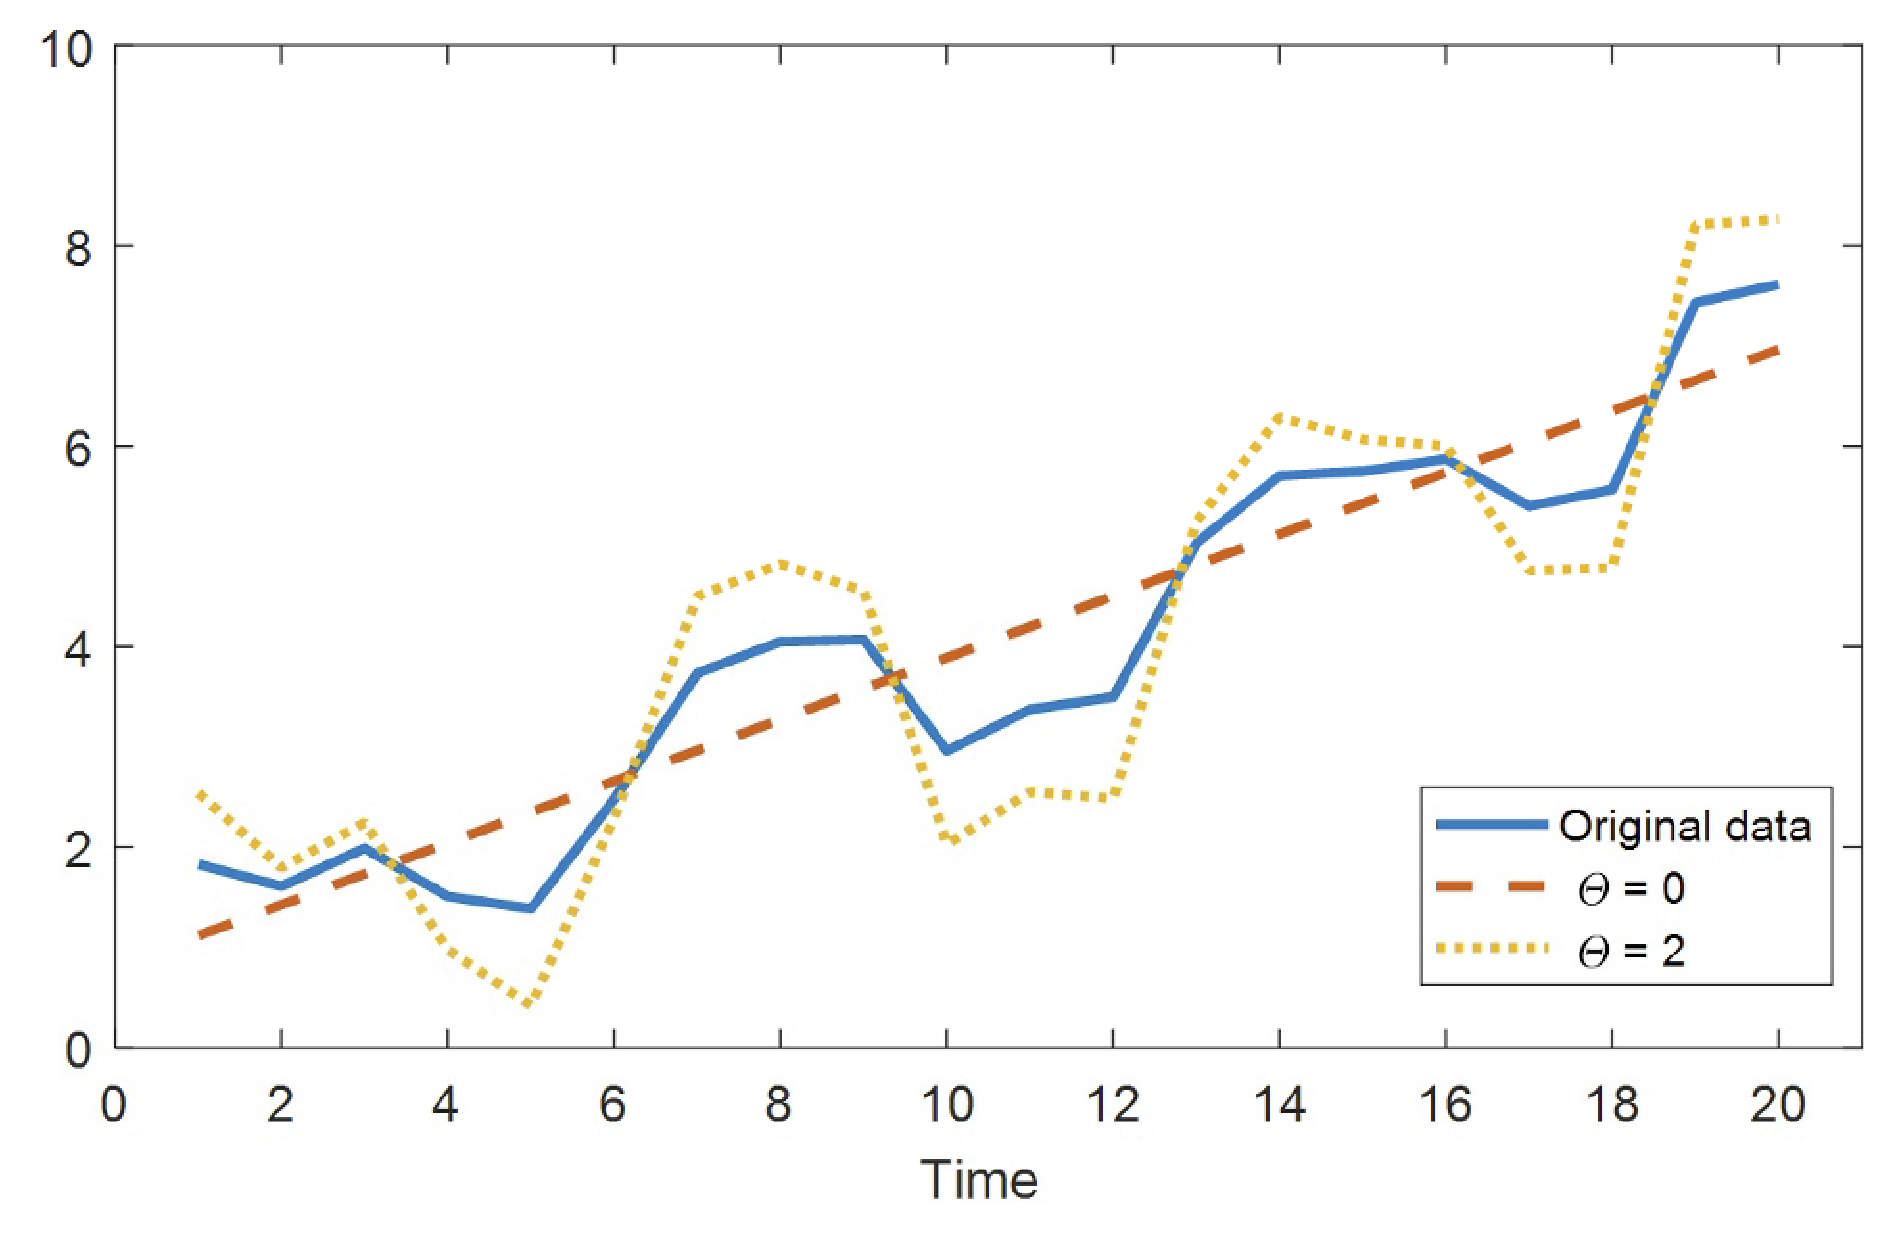
\includegraphics[width=0.6\textwidth]{theta.png}
\caption{The canonical ``Theta lines'', from \citet{dudek2019short}.}      
\label{fig:theta}
\end{figure}

\item \citet{hyndman2003unmasking} show that this procedure is quite similar to
  running SES with an added linear trend, whose slope is \smash{$\hat{b}_0 /
    2$}. This is like a special case of Holt's linear trend method with $\beta =
  0$ (no evolution of the slope over time)   

\item These authors also compare the Theta method with Holt's linear trend
  method on the data from the M3 forecasting challenge (where the Theta method
  performed well and was subsequently thrown into the spotlight), and observe
  that Holt's linear trend performs competitively  

\item It is worth knowing about the close connections between Theta and
  exponential smoothing, as much of the literature on the Theta model does not
  seem to emphasize this aspect. There has been more recent work on the Theta
  model (which may further distinguish it from exponential smoothing---we cannot
  say, because we have not followed it) that you may be interested in reading up
  on    
\end{itemize}

\subsection{Prophet model}

\begin{itemize}
\item Next on our list is the \emph{Prophet model}, proposed by
  \citet{taylor2018forecasting}, from Facebook/Meta. This has become popular for 
  large-scale forecasting enterprises, and the popular opinion seems to be that
  its advantages over traditional ARIMA or ETS models are twofold: flexibility
  and speed. But, make sure to read on, especially to the end of this
  subsection, for further discussion of this  

\item The Prophet model is a particular type of signal plus noise model, 
  \[
  x_t = g_t + s_t + h_t + \epsilon_t
  \]
  where $\epsilon_t$, $t = 1,2,3,\dots$ is a white noise sequence, and:
  \begin{itemize}
  \item $g_t$ represents a trend component
  \item $s_t$ represents a seasonal component
  \item $h_t$ captures holiday/calendar effects 
  \end{itemize}

\item This can be seen as a particular type of smoother, based on a particular
  model for the trend (which we will describe shortly; the seasonal and holiday
  components are fairly generic). We could also refer to it as a particular type
  of additive model, where the regressor is time

\item The seasonal component is parametrized by a Fourier (cosine and sine)
  basis at given fixed, known periods chosen by the user. For frequencies
  $\omega_j$, $j = 1,\dots,p$ (equivalently, periods $1/\omega_j$, $j =
  1,\dots,p$), recall, this is:  
  \[
  s_t = \sum_{j=1}^p \Big( a_j \cos(2\pi \omega_j t) + b_j \sin(2\pi \omega_j t)
  \Big) 
  \]
  for coefficients $a_j, b_j$, $j = 1,\dots,p$

\item The holiday/calendar component is simply parametrized using indicator
  variables 
  \[
  h_t = \sum_{j=1}^m \alpha_j \cdot 1\{ t \in D_j \}
  \]
  where $\alpha_j$, $j = 1,\dots,m$ are coefficients and each $D_j$ is a set of
  dates representing a particular holiday or calendar event (e.g., Christmas,
  Thanksgiving, etc.) 

\item Finally, the trend component is modeled in one of two ways. The first way
  is for \emph{saturating} trends. For this, \citet{taylor2018forecasting}
  propose to model $g_t$ using a sigmoid function with a piecewise growth rate:  
  \[
  g_t = \frac{C(t)}{1 + \exp\Big( -c_0 - c_1 t - \sum_{j=1}^r \beta_j \cdot
    (t-t_j)_+\Big)}  
  \]
  where $u_+ = \max\{u,0\}$ denotes the positive-part of $u$.
  Here $C(t)$ is a (possibly) time-varying capacity, which it appears 
  \citet{taylor2018forecasting} recommend be set externally (e.g., based on  
  market size considerations)

\item For \emph{non-saturating} trends, \citet{taylor2018forecasting}
  propose to model $g_t$ using a piecewise linear trend directly: 
  \[
  g_t = c_0 + c_1 t + \sum_{j=1}^r \beta_j \cdot (t-t_j)_+ 
  \]

\item In either case (saturating or non-saturating), $\beta_j$, $j = 1,\dots,r$
  are coefficients to be estimated. Also, $t_j$, $j = 1,\dots,r$ are knots
  (locations where the slope changes), which, in the simplest case, could be
  fixed ahead of time. Instead, \citet{taylor2018forecasting} recommend that
  knots be selected using $\ell_1$ penalization from a large initial set of 
  locations. That is, they use the $\ell_1$ penalty 
  \[
  \sum_{j=1}^r |\beta_j|
  \]
  when fitting the model, which is like a special type of lasso regression. (In
  fact, though it may not be obvious at first pass, placing an $\ell_1$ penalty
  on $\beta_j$, $j = 1,\dots,r$ here is actually equivalent to reparametrizing
  the entire sequence as $g_t = \theta_t$, and then using an $\ell_1$ penalty on  
  second differences of $\theta_t$; recall, this is the penalization scheme used
  in \emph{trend filtering}, which you learned earlier in the course when we
  covered smoothing)   

\item Altogether, the Prophet model is fit by minimizing the sum of squared
  errors to the observed data, over all parameters
  $a_j,b_j,\alpha_j,c_0,c_1,\beta_j$ that determine the decomposition, with a
  squared $\ell_2$ (ridge) penalty on the parameters $a_j,b_j,\alpha_j$ for the
  seasonal component $s_t$ and holiday component $h_t$, and an $\ell_1$ (lasso)
  penalty on the parameters $\beta_j$ for the trend component $g_t$  

\item Forecasts are generated by extrapolating the fitted components forward in 
  time. For $s_t$ and $h_t$, this is straightforward, because they are periodic
  in nature. For $g_t$, this is done by holding the slope (i.e., growth rate in
  the saturating model) constant from its last value, as we move forward in
  time 

\item (Though unimportant for our purposes here, \citet{taylor2018forecasting}
  actually phrase all of this in the context of a hierarchical Bayesian model,
  with normal and Laplace priors that serve the purpose of regularization;  
  this Bayesian machinery also provides added stochasticity in computation of 
  prediction intervals) 

\item So, how does the Prophet model compare to ARIMA and ETS? It depends on who
  you ask. In their original paper, \citet{taylor2018forecasting} find that
  ARIMA and ETS models are too rigid in their motivating examples---take a look
  at Figure 3 in their paper, and compare Figure \ref{fig:prophet}, which
  displays Prophet forecasts on the same data

\begin{figure}[htb]
\centering
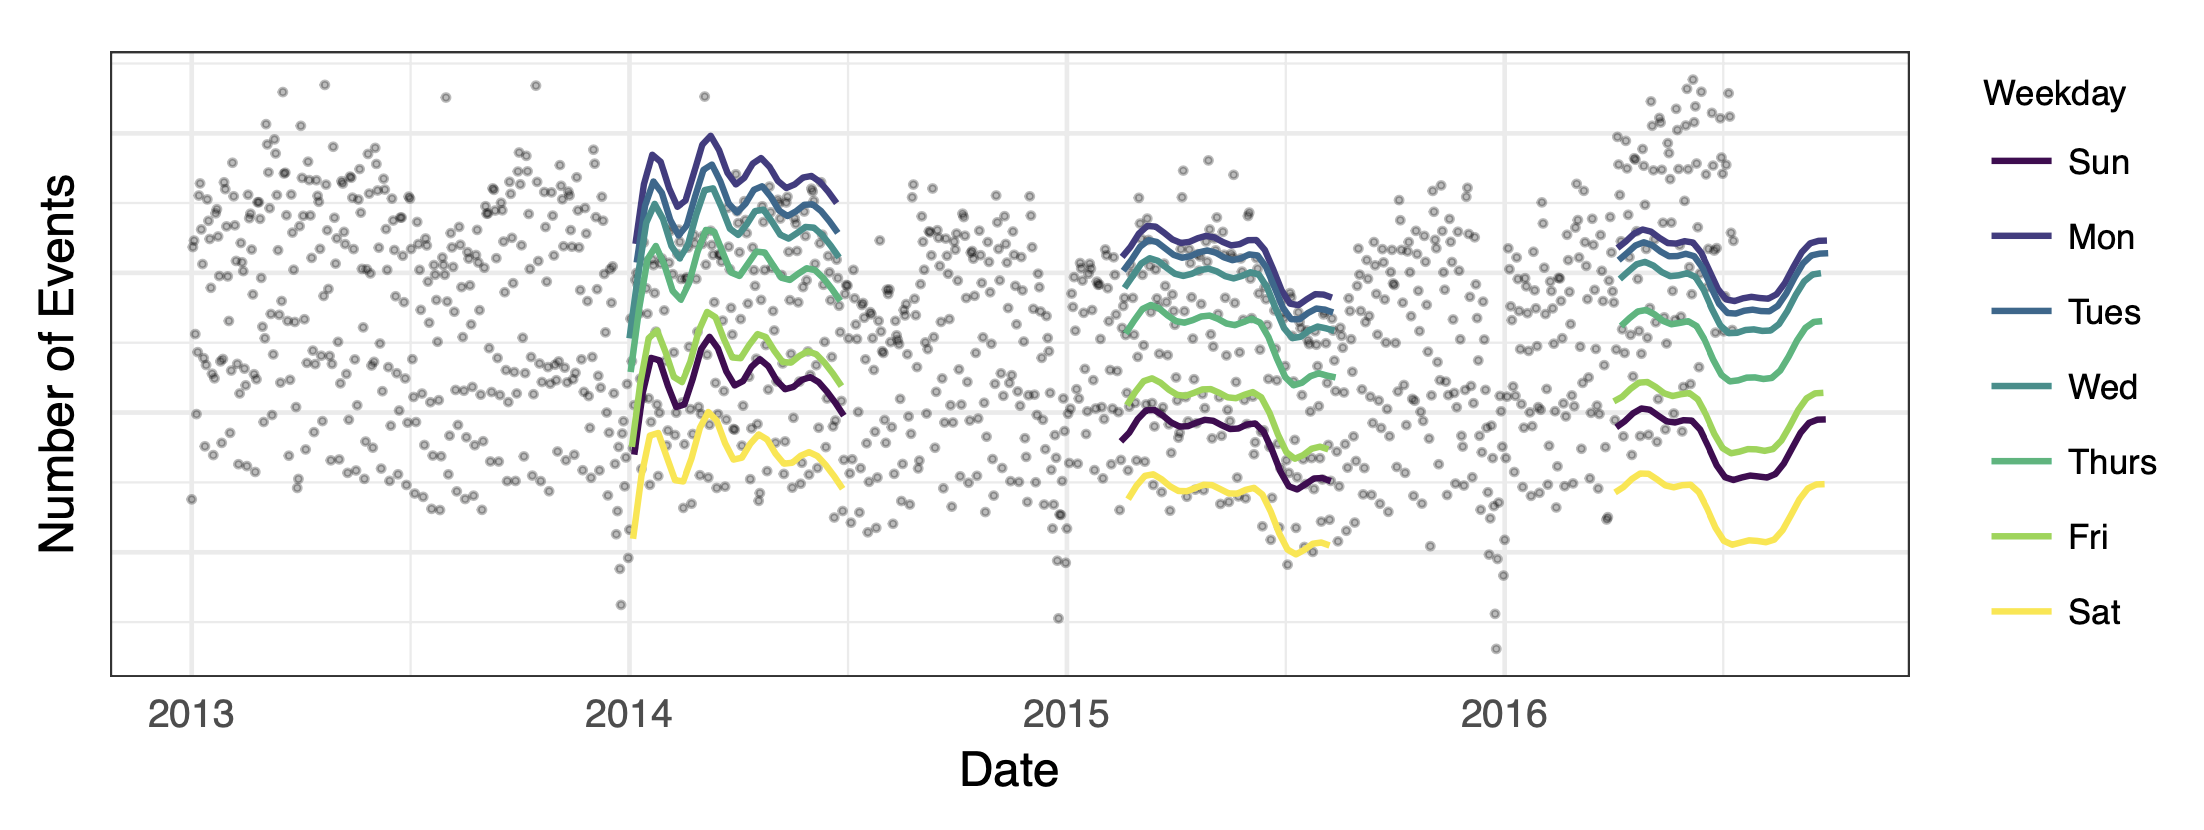
\includegraphics[width=0.95\textwidth]{prophet.png}
\caption{Prophet forecasts, from \citet{taylor2018forecasting}.}
\label{fig:prophet}
\end{figure}

\item Indeed, in their traditional forms, ARIMA and ETS models lack the
  flexibility of the Prophet model, particularly the flexibility exhibited in
  the latter's trend component. However, both ARIMA and ETS can be extended to
  accommodate more sophisticated trends. With ARIMA, you have actually already
  seen a way to do this: we can phrase the problem as \emph{regression with
    correlated errors} (where we use an ARIMA model for the errors), and then
  use a flexible basis representation to model trends just like Prophet does. As
  a reminder, this model takes the form     
 \[
  x_t = \sum_{j=1}^k u_{tj} b_j + z_t, \quad t = 1,\dots,n
  \]
  where $z_t$, $t = 1,\dots,n$ follows an ARIMA($p,d,q$) model. To capture the
  same model as Prophet, we could simply define one feature $u_{tj}$ per cosine
  and sine basis function $\cos(2\pi \omega_j t)$ and $\sin(2\pi \omega_j t)$,
  one feature per holiday indicator $1\{ t \in D_j\}$, and one feature per
  piecewise linear function $(t-t_j)_+$  

\item Hyndman and Athanasopoulos (HA) call this a \emph{dynamic regression
    model} and study it in Chapter 10 of their book. The advantage this has over 
  Prophet is that it is able to capture auto-correlations in the errors, which
  can lead to narrower prediction intervals. The advantage Prophet has is speed:
  it is usually more efficient to fit the Prophet model, since its error model
  (white noise) is simpler and this makes optimization easier 
\end{itemize}

\subsection{Neural network autoregression}

\begin{itemize}
\item A \emph{neural network} describes a class of models that make real-valued
  predictions $f(x) \in \R$ from an input feature vector $x \in \R^p$ of the
  form:  
  \begin{align*}
  f_1(x) &= \rho(W_1 x + b_1) \\
  f_\ell(x) &= \rho \Big( W_{\ell-1} f_{\ell-1}(x) + b_{\ell-1} \Big), \quad
              \ell = 2,\dots,L \\
  f(x) &= f_L(x)
  \end{align*}

\item Here each $W_\ell \in \R^{d_\ell \times d_{\ell-1}}$ is a matrix of
  weights that maps from the dimension $d_{\ell-1}$ of layer $\ell-1$ to the
  dimension $d_\ell$ of layer $\ell$. Note that $d_0 = p$, and $d_L = 1$ (for
  real-valued predictions)

\item Each $b_\ell \in \R^{d_\ell}$ is a vector of intercepts (often called
  \emph{biases} in the deep learning community). Generically, the parameters
  $W_\ell,b_\ell$ are all learned by minimizing the sum of squared errors of
  predictions on the training data 

\item The function $\rho$ is a nonlinear \emph{activation function} that is 
  interpreted as being applied componentwise. It is user-chosen; common choices 
  are $\rho(u) = u_+$ and $\rho(u) = 1/(1+e^{-u})$

\item Lastly, $L$ here is the number of layers, also a design choice, and often 
  called the \emph{depth} of the network   

\item For time series, one of the simplest things that can be done with neural
  networks is just to form input features by taking lags of the given response
  variable. We can use both nonseasonal and seasonal lags (as in ARIMA). This
  gives rise to what we call a \emph{neural network autoregressive} (NNAR) model  

\item What we described above is actually just a particular type of neural
  network architecture, and indeed, the simplest kind, called a
  \emph{feedforward} neural network. Many other architectures are possible, and
  some more appropriate for time series data, such as the \emph{long short term
    memory} (LSTM) network, a type of recurrent neural network

\item A popular time series forecaster based on LSTMs is called \emph{DeepAR},
  proposed by \citet{salinas2020deep}, from Amazon. Relative to all other
  methods you have learned thus far, DeepAR is quite complicated to describe
  precisely (and to train). Figure \ref{fig:deepar} gives a schematic: the left
  column for training, and the right for forecasting

\begin{figure}[htb]
\centering
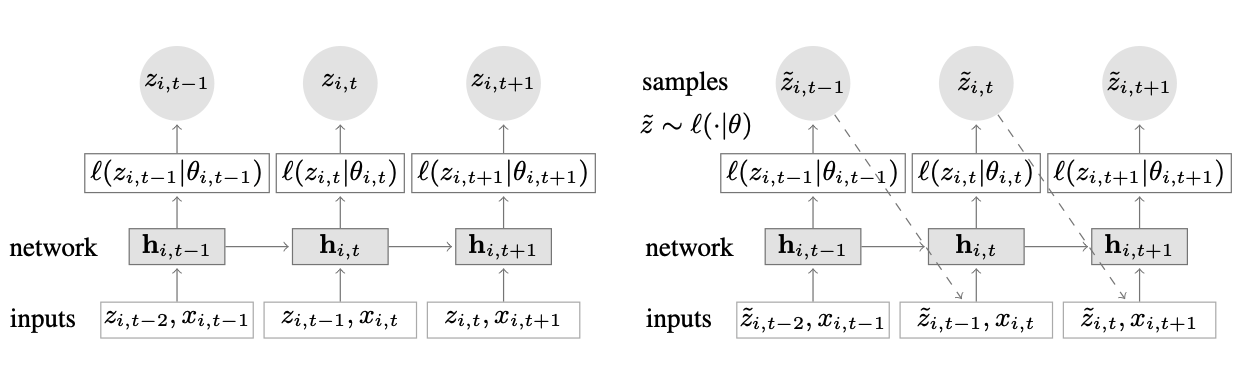
\includegraphics[width=0.95\textwidth]{deepar.png}
\caption{Schematic of DeepAR network, from \citet{salinas2020deep}, where each
  $h_{i,t}$ is the output of a recurrent neural network with LSTM cells.} 
\label{fig:deepar}
\end{figure}

\item DeepAR can work very well in data-rich prediction problems which have a 
  high signal-to-noise ratio, but it can also be too variable outside of these
  settings, as can other deep learning forecasters  

\item A strength DeepAR is are often cited as having is that it can learn rich,
  joint correlation structures between \emph{multiple} time series---think of  
  spatiotemporal data, where we have one time series per location, and many 
  locations---and it can and produce forecasts which respect this correlation
  structure 

\item You'll also often hear people saying that ARIMA or ETS models are
  incapable of modeling multiple series. From the traditional point-of-view this
  is true. There are extensions of these models to handle multiple series, for
  example, \emph{vector autoregressive} (VAR) models. However, these models are
  typically too cumbersome to fit at large scale, when we have many time series
  we want to co-model. A simpler alternative would be run ARIMA or ETS
  individually on each time series of interest, and then model the dependence in 
  their forecasts errors as a second-layer model, whose output we could use to 
  adjust the original forecasts

\item Finally, and perhaps unsurprisingly, many researchers are now re-purposing
  transformers in order to turn them into time series forecasters. As deep 
  learning continues to move forward, we will continue to see spillover into
  time series forecasting   
\end{itemize}

\section{Ensembling}

\begin{itemize}
\item So, you have lagged regression, ARIMA, ETS, Theta, Prophet, and DeepAR in
  your forecast toolkit. You have data in front of you, and you're unsure which
  model(s) will work best. What do you do?    

\item The answer we have given all semester: \emph{use time series CV}. That is,
  move the time index back to $t = t_0$, train each model on the past, make 
  forecasts, compare to the unseen target values, march the time index forward
  sequentially, and repeat. In doing so, we can compute our chosen accuracy
  metric (MAE, MASE, etc.) for each model, and choose the one that emerges as 
  the most accurate, perhaps using Occam's razor to help decide between models
  that perform similarly

\item Here is an alternative that can often be advantageous: \emph{combine} the
  models, which can be informed by their out-of-sample predictions from time 
  series CV, rather than using CV to select one of them
  
\item The combination of prediction models is often called \emph{ensembling}, or
  \emph{aggregation}. It has a long history in statistics and machine learning,
  including in forecasting. Still, it seems perhaps people don't quite
  appreciate enough just how effective it can be

\item Roughly speaking, there are two types of ensembles: \emph{untrained} and
  \emph{trained} ones. An untrained ensemble simply combines a given set of 
  base models (also called constituent models) without consideration of
  their individual past performance. Meanwhile, a trained ensemble combines the
  base models in a way that reflects their performance, typically upweighting
  more accurate base models 

\item At a high level, an ideal ensemble model would satisfy the following two
  properties:
  \begin{enumerate}
  \item ``compete-with-best'': the ensemble should have competitive accuracy
    with the best indvidual constituent model  
  \item ``robustness-over-all'': the ensemble should have superior robustness 
    (make fewer large errors) than any individual constituent model  
  \end{enumerate}

\item Interestingly, these two properties appear to be somewhat at odds.
  Untrained ensembles can be \emph{very} robust, but typically cannot compete
  with the best constituent model. On the other hand, trained ensembles can
  compete with the best constituent model (and even outperform it, if the
  ensemble is flexible enough), but ``heavier'' training schemes tend to hurt
  robustness  
\end{itemize}

\subsection{Untrained methods}

\begin{itemize}
\item The simplest untrained ensemble method is just to take a straight average
  of all constituent model forecasts. Denote these by
  \smash{$\hat{x}^j_{t+h|t}$}, for $j = 1,\dots,p$. Then the simple average
  ensemble forecast is 
  \[
  \hat{x}^{\text{avg}}_{t+h|t} = \frac{1}{p} \sum_{j=1}^p \hat{x}^j_{t+h|t} 
  \] 

\item Another option is to take a median of point forecasts from the constituent
  models,
  \[
  \hat{x}^{\text{med}}_{t+h|t} = \mathrm{median}\Big\{ \hat{x}^j_{t+h|t} : j =
  1,\dots,p \Big\} 
  \]

\item Despite their simplicity, these methods can be very effective, especially
  when we have a diverse set of constituent models (which have a healthy degree
  of diversity in their errors), as this can lead to very robust average or
  median ensembles

\item Figure \ref{fig:cramer} shows a striking example of this, from 1- though
  4-week ahead Covid-19 death forecasting. The COVIDhub-ensemble model was (for
  most of the pandemic) a simple median ensemble of all forecasts submitted to
  the US Covid-19 Forecast Hub which met a certain very basic set of inclusion
  criteria (ruling out wild or unrealistic forecasts). This ensemble model was
  the basis for all official CDC communications on short-term Covid-19
  forecasting. The number of constituent models fluctuated up and down over
  time, in between about 25 to 50   

\item For state-level forecasts made over a 1.5 year period during the pandemic, 
  the figure considers a notion called \emph{standardized rank} that is defined
  as follows. For a given forecast task (given state, given target date, and
  given horizon), we rank all available forecasts using an accuracy measure
  called WIS (a generalization of absolute error for quantile-based forecasts)
  figure. We assign a standardized rank of 1 for the most accurate forecast of
  all available forecasts for that task, and 0 to the least accurate. Then for
  each forecaster, we plot a histogram of their standardized rank distribution
  over all tasks  

\item As we can see in Figure \ref{fig:cramer}, the distribution of the ensemble is
  \emph{very} different from all others---in particular, look at its thin left
  tail. It is the only forecast model that was in the top half of forecasters 
  (standardized rank $\geq 0.5$) for 75\% of the forecast tasks. Interestingly,
  we can also see that it is not in the top quartile of forecasters
  (standardized rank $\geq 0.75$) as often as the best constituent models,
  hinting at the tradeoff described above  

\begin{figure}[htb]
\centering
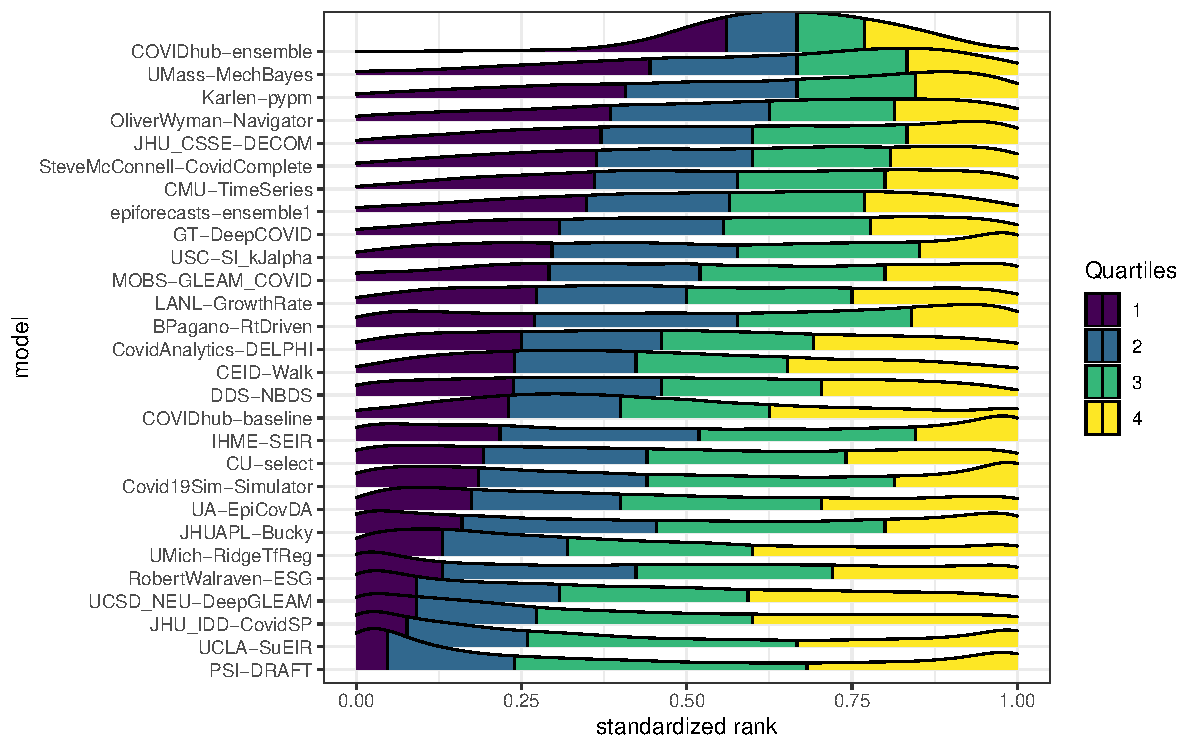
\includegraphics[width=\textwidth]{cramer.pdf}
\caption{Comparison of Covid-19 death forecast models, from
  \citet{cramer2022evaluation}.}    
\label{fig:cramer}
\end{figure}
\end{itemize}

\subsection{Trained methods}

\begin{itemize}
\item One of the simplest trained ensemble methods is to directly fit a weighted 
  combination of constituent forecasts in order to optimize accuracy (MSE, MAE,
  etc.). For example, going by MSE, and fixing $h=1$ for simplicity, to form the
  ensemble at time $t$ (for a forecast of the target value at time $t+1$), we
  would first solve:
  \begin{alignat*}{2}
  &\min_{w \in \R^p} && \hspace{-6pt} \sum_{s=t_0+1}^t \bigg( x_s - \sum_{j=1}^p
  w_j \cdot \hat{x}^j_{s|s-1} \bigg)^2 \\   
  &\st \quad && \sum_{j=1}^p w_j = 1, \;\;\text{and} \;\; w_j \geq 0, \;
  j=1,\dots,p   
  \end{alignat*}
  Note that this is simply a regression of the target values (response) on the
  forecasts made by constituent models (features), where we constrain the
  coefficients to be nonnegative and sum to 1

\item After obtaining the solution \smash{$\hat{w}^t_j$}, $j = 1,\dots,p$, we
  then form the weighted ensemble to make forecasts 
  \[
  \hat{x}^{\text{stack}}_{t+1|t} = \sum_{j=1}^p \hat{w}^t_j \cdot
  \hat{x}^j_{t+1|t} 
  \]

\item This is sometimes called \emph{linear stacking}: here ``stacking'' refers
  to the fact that we have stacked the predictions made by our constituent
  models into features for a second-level model, and ``linear'' refers to the
  fact that our second-level model is linear in the features (it is a linear
  regression subject to constraints)  

\item Instead of re-solving the optimization problem above at each forecast time
  $t$, we could also incrementally update the learned weights over time. An
  algorithm called (online) \emph{mirror descent} applied to the above
  optimization problem yields the following intuitive weight updates, at time
  $t$:     
  \begin{align*}
  \tilde{w}^t_j &= \hat{w}^{t-1}_j \exp\bigg\{ \eta \cdot \hat{x}^j_{t|t-1}
    \bigg( x_t -  \sum_{j=1}^p \hat{w}^{t-1}_j \cdot \hat{x}^j_{t|t-1} \bigg)
    \bigg\}, \quad j = 1,\dots,p \\
  \hat{w}^t_j &= \tilde{w}^t_j \bigg/ \sum_{\ell=1}^p \tilde{w}^t_\ell, \quad j =
    1,\dots,p 
  \end{align*}
  Here $\eta > 0$ is a parameter called the learning rate. In words, if a
  forecaster's latest prediction \smash{$\hat{x}^j_{t|t-1}$} is correlated with
  the ensemble's latest residual \smash{$x_t -  \sum_{j=1}^p \hat{w}^{t-1}_j
    \cdot \hat{x}^j_{t|t-1}$}, then it is underrepresented in the ensemble, and
  we increase its weight. This is related to a general class of online learning 
  algorithms called \emph{exponential weights} algorithms; and there is a 
  huge literature on related schemes

\item Stacking---especially more flexible second-level models which are
  nonlinear or use weights that depend on features---can lead to impressive
  accuracy in practice. Figure \ref{fig:fakoor} shows a nice example of this
  (albeit in a batch prediction context, rather than time series). The figure
  shows a neural network ensemble model called \emph{deep quantile aggregation}
  (DQA), that is trained as a second-layer model on top of many constituent
  models, including some very flexible ones (such as deep neural
  networks). Across 35 data sets, ordered by their signal-to-noise ratio along 
  the x-axis, the WIS (recall this is a generalization of absolute error for
  quantile-based predictions) of all of the constituent models and other
  ensemble methods is compared to that of DQA. We can see that no method
  outperforms DQA (nothing below the red horizontal line), and for problems with
  more signal, towards the right end of the x-axis, DQA improves massively on a
  lot of the other models   

\begin{figure}[htb]
\centering
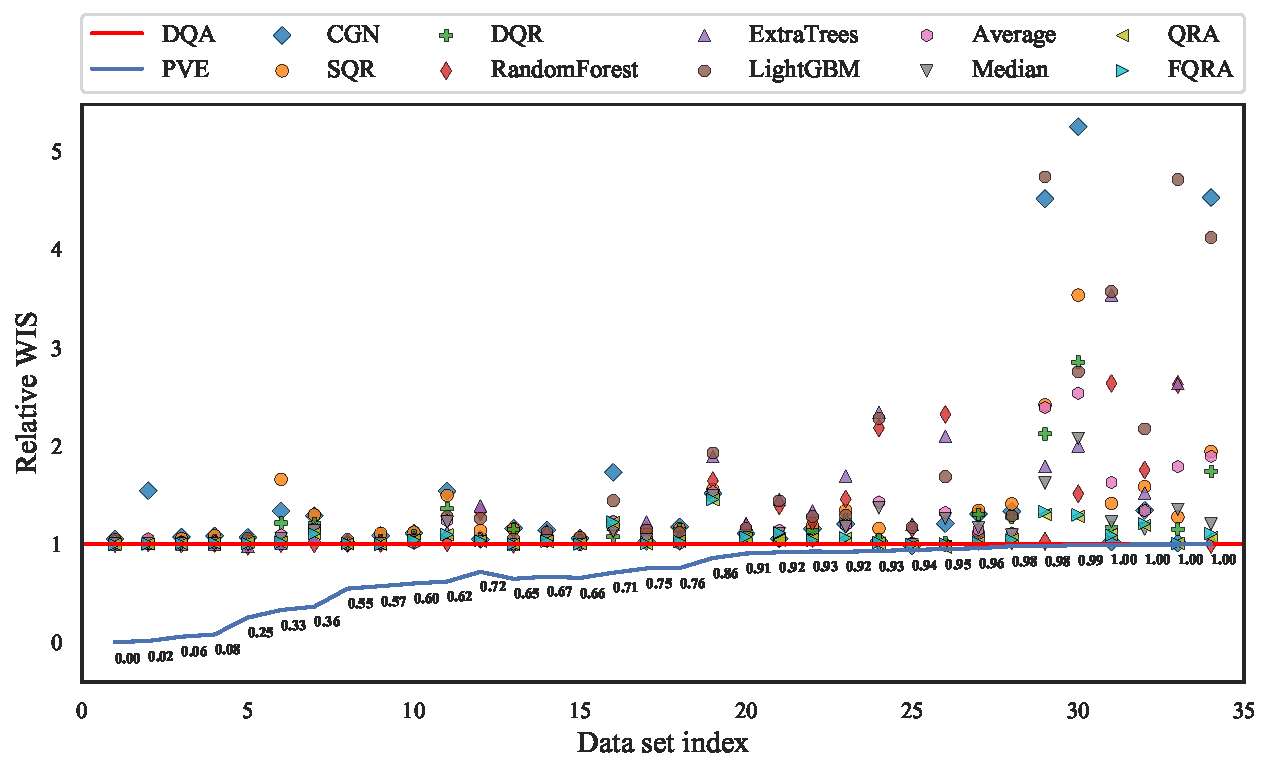
\includegraphics[width=\textwidth]{fakoor.pdf}
\caption{Deep stacking of quantile prediction models, from 
  \citet{fakoor2023flexible}.}   
\label{fig:fakoor}
\end{figure}
\end{itemize}

\section{Calibration}

\begin{itemize}
\item Beyond point forecasts, all of the methods that we have learned thus far
  produce \emph{prediction intervals}, which reflect uncertainty in the
  predictions that are made, useful for downstream decision-making   

\item How can we measure the ``fidelity'' of such prediction intervals? Fixing a
  horizon $h$, denote by \smash{$I^{1-\alpha}_ {t+h|t}$} denote the level
  $1-\alpha$ prediction interval made by our forecaster at time $t$, for the
  target variable $x_{t+h}$ at time $t+h$. For (say) a 90\% prediction interval,
  this is often (though not necessarily) of the form: 
  \[
  I^{1-\alpha}_{t+h|t} = 
  \big[\hat{x}_{t+h|t} - \hat\sigma_h q_{0.95}, \, \hat{x}_{t+h|t} +  
  \hat\sigma_h q_{0.95} \big]
  \]
  where \smash{$\hat{x}_{t+h|t}$} is a point forecast of $x_{t+h}$ made a time
  $t$, \smash{$\hat\sigma^2_h$} is an estimate of the variance of the $h$-step  
  ahead forecast distribution, and $q_{0.95}$ is the 0.95 quantile of the
  standard normal distritbuion  

\item Given such intervals, we can measure their empirical \emph{coverage}, in a
  time series CV sense:  
  \[
  \mathrm{Coverage} = \frac{1}{n-t_0} \sum_{t=t_0+1}^n 1\big\{ x_t \in 
  I^{1-\alpha}_{t|t-h} \big\}
  \]
  In words, this the fraction of times that our prediction intervals cover their
  targets

\item Of course, we want the coverage of our prediction intervals to roughly
  match the nominal level, 
  \[
    \frac{1}{n-t_0} \sum_{t=t_0+1}^n 1\big\{ x_t \in I^{1-\alpha}_{t|t-h} \big\}
    \approx 1-\alpha
  \]
  increasingly so for large $n$

\item Sadly, traditional methods for producing prediction intervals will not
  always yield empirical coverage that hovers around the nominal level. This is 
  because the methods for producing these intervals rely on assumptions that are
  often violated in practice

\item See Figure \ref{fig:reich} for an example of the empirical coverage of
  the COVIDhub-ensemble model for forecasting cases, hospitalizations, and
  deaths. These are very difficult forecasting problems (especially cases and
  hospitalizations)    

\begin{figure}[htb]
\centering
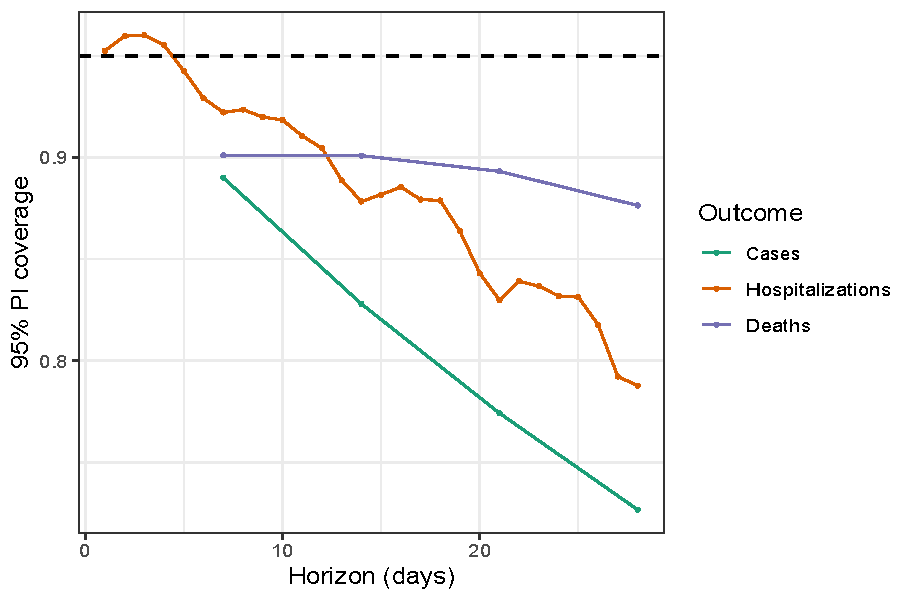
\includegraphics[width=0.8\textwidth]{reich.pdf}
\caption{Empirical coverage of Covid-19 ensemble forecasts, from
  \url{https://delphi.cmu.edu/blog/2021/09/30/on-the-predictability-of-covid-19/}.} 
\label{fig:reich}
\end{figure}

\item In what remains, we'll learn about a simple and generic method for
  adjusting prediction intervals online, so that their empirical coverage tracks
  the nominal level more faithfully. Then we'll learn about how to generalize
  the concept of coverage (which applies to a prediction interval) so that we
  can measure the fidelity of an entire predicted distribution. This brings us
  to a topic called \emph{calibration}  
\end{itemize}

\subsection{Quantile tracking}

\begin{itemize}
\item We briefly describe a method due to \citet{angelopoulos2023conformal},
  called \emph{quantile tracking}. Fix $h=1$ for simplicity, and suppose
  \smash{$\hat{q}^{1-\alpha}_t$} were an estimated level $1-\alpha$ quantile of
  the distribution of $e_t$, the absolute forecast error at time $t$:   
  \[
  e_t = \big| x_t - \hat{x}_{t|t-1} \big|
  \]

\item Note that a level $1-\alpha$ prediction interval for $x_t$ could then be
  formed via: 
  \[
  I^{1-\alpha}_{t|t-1} = \big[ \hat{x}_{t|t-1} - \hat{q}^{1-\alpha}_t, \,
  \hat{x}_{t|t-1} + \hat{q}^{1-\alpha}_t \big]
  \]

\item The motivation is as follows: \smash{$e_t \leq \hat{q}^{1-\alpha}_t \iff
    x_t \in I^{1-\alpha}_{t|t-1}$}, so if \smash{$\hat{q}^{1-\alpha}_t$} were a
  proper level $1-\alpha$ quantile in the long-run frequency sense:
  \[
  \frac{1}{T} \sum_{t=t_0+1}^{t_0+T} 1 \big\{ e_t \leq \hat{q}^{1-\alpha}_t
  \big\} \approx 1-\alpha
  \]
  for large $T$,  then we would indeed have empirical coverage: 
  \[
  \frac{1}{T} \sum_{t=t_0+1}^{t_0+T} 1 \big\{ x_t \in
    I^{1-\alpha}_{t|t-1} \big\} \approx 1-\alpha
  \]
  for large $T$

\item \citet{angelopoulos2023conformal} propose the following online quantile 
  update: 
  \[
  \hat{q}^{1-\alpha}_{t+1} =
  \begin{cases}
  \hat{q}^{1-\alpha}_t + \eta (1-\alpha) & \text{if $x_t \notin
    I^{1-\alpha}_{t|t-1}$} \\ 
  \hat{q}^{1-\alpha}_t - \eta \alpha & \text{if $x_t \in I^{1-\alpha}_{t|t-1}$}  
  \end{cases}
  \]
  where $\eta > 0$ is a parameter called the learning rate. In words, if the
  latest interval does not cover, then we \emph{increase} the quantile by 
  $\eta(1-\alpha)$ (make the next interval \emph{wider}), whereas if the latest 
  interval covered, then we \emph{decrease} the quantile by $\eta\alpha$ (make
  the next interval \emph{narrower})

\item This is very intuitive, and it turns out to be equivalent to online
  gradient descent run on a particular loss function (which sums the quantile
  loss between $e_t$ and \smash{$\hat{q}^{1-\alpha}_t$} over all time $t$). See
  also \citet{gibbs2021adaptive} for an earlier, related idea which inspired the
  quantile tracking work

\item \citet{angelopoulos2023conformal} prove that if the forecast errors are
  bounded, $e_t \leq b$ for all $t$ and for some $b < \infty$ (note that we do
  not need to know the bound $b$ in order to run the algorithm), then quantile 
  tracking results in long-run coverage: 
  \[
  \frac{1}{T} \sum_{t=t_0+1}^{t_0+T} 1 \big\{ x_t \in I^{1-\alpha}_{t|t-1}
  \big\} \to 1-\alpha, \quad \text{as $T \to \infty$} 
  \]
  for any $t_0$ and $\eta$. Importantly, this holds \emph{with no assumptions}
  on the distribution of the data or the forecast errors (or the forecaster
  itself)

\item Note: we do not need to use absolute errors, we could use \emph{signed}
  errors and fit the upper and lower endpoints of the prediction intervals
  separately (to allow for asymmetry around the point forecast) 

\item Another important note: we do not need to start with point forecasts. We
  could start with the endpoints of a prediction interval produced by
  traditional methods, and iteratively adjust these to have proper coverage.
  This will typically be more effective than using errors around a point
  forecast, since the required adjustment will typically be more minor once we
  start from the interval endpoints 

\item In more detail, denote by \smash{$[\ell^{\alpha/2}_{t|t-1}, \,
    u^{1-\alpha/2}_{t|t-1}]$} an equi-tailed level $1-\alpha$ prediction
  interval produced by a traditional method (like what you learned in the ARIMA
  or ETS lectures). Quantile tracking can be used to adjust each of these
  endpoints individually to have proper one-sided coverage. We want:  
  \[
  \frac{1}{T} \sum_{t=t_0+1}^{t_0+T} 1 \big\{ x_t \leq \hat\ell^{\alpha/2}_t 
  \big\} \approx \alpha/2 \quad \text{and} \quad
  \frac{1}{T} \sum_{t=t_0+1}^{t_0+T} 1 \big\{ x_t \leq \hat{u}^{1-\alpha/2}_t   
  \big\} \approx 1-\alpha/2
  \]
  for large $T$. Then we would indeed have empirical coverage: 
  \[
  \frac{1}{T} \sum_{t=t_0+1}^{t_0+T} 1 \big\{ x_t \in [ \hat\ell^{\alpha/2}, \, 
  \hat{u}^{1-\alpha/2}] \big\} \approx 1-\alpha    
  \]
  for large $T$. To form the adjustments \smash{$\hat\ell^{\alpha/2}, \, 
    \hat{u}^{1-\alpha/2}$}, we track the $\alpha/2$ quantile of
  \smash{$e^\text{lo}_t = x_t - \ell^{\alpha/2}_{t|t-1}$} and $1-\alpha/2$ 
  quantile of \smash{$e^\text{up}_t = x_t - u^{1-\alpha/2}_{t|t-1}$}, 
  respectively. For the lower endpoint adjustment, we define 
  \[
    \hat\ell^{\alpha/2}_{t+1} = \ell^{\alpha/2}_{t+1|t} +
    \hat{q}^{\alpha/2}_{t+1}  
  \] 
  where \smash{$\hat{q}^{\alpha/2}_{t+1}$} itself is defined via the iteration   
   \[
  \hat{q}^{\alpha/2}_{t+1} =
  \begin{cases}
  \hat{q}^{\alpha/2}_t + \eta \alpha/2 & \text{if $x_t >
    \hat\ell^{\alpha/2}_{t+1}$} \\  
  \hat{q}^{\alpha/2}_{t+1} - \eta (1-\alpha/2) &\text{if $x_t \leq  
    \hat\ell^{\alpha/2}_{t+1}$}  
  \end{cases}
  \]
  and similarly for the upper endpoint, we define 
  \[
    \hat{u}^{1-\alpha/2}_{t+1} = u^{1-\alpha/2}_{t+1|t} +
    \hat{q}^{1-\alpha/2}_{t+1}  
  \] 
  where \smash{$\hat{q}^{1-\alpha/2}_{t+1}$} itself is defined via the iteration    
   \[
  \hat{q}^{1-\alpha/2}_{t+1} =
  \begin{cases}
  \hat{q}^{1-\alpha/2}_t + \eta (1-\alpha/2) & \text{if $x_t >
    \hat{u}^{1-\alpha/2}_{t+1}$} \\ 
  \hat{q}^{1-\alpha/2}_{t+1} - \eta \alpha/2 &\text{if $x_t \leq
    \hat{u}^{1-\alpha/2}_{t+1}$}  
  \end{cases}
  \]

\item You can read the paper for more (extensions to handle unbounded scores,
  and prospective corrections to forecast errors, driven by a connection to
  control theory)     
\end{itemize}

\subsection{PIT calibration}

\begin{itemize}
\item Last but not least, we arrive at calibration. Unfortunately, this is a
  term that is often used ambiguously, to mean different things. Here we use  it
  to mean a precise way of measuring the fidelity of an entire \emph{predicted
    distribution}, rather than just a prediction interval  

\item That is, suppose that our forecaster produces an entire distribution
  $F_{t|t-h}$ for the target $x_t$ at time $t$. Generally, we think of
  $F_{t|t-h}$ as a cumulative distribution function (CDF); note that, from
  $F_{t|t-h}$, we could obviously produce prediction intervals for $x_t$ (at any
  levels that we desire)

\item For notational simplicity, we will hide the forecast time $t-h$, and
  simply denote the predicted distribution $F_{t|t-h}$ by $F_t$ in what follows 

\item Now, there are numerous different definitions of what it means for a
  probabilistic forecaster (which produces $F_t$) to be calibrated, and these
  definitions are not generally equivalent. (This contributes to the frequent
  ambiguity in the use of the term ``calibration''.) See, e.g.,
  \citet{gneiting2023regression} for a recent nice overview of different
  definitions and their relationships

\item We will stick with one particular definition. The forecaster that produces
  the sequence of predicted CDFs $F_t$ is said to be \emph{PIT calibrated}
  provided:  
  \begin{multline*}
  \text{the empirical distribution of $F_t(x_t)$, $t = 1,\dots,T$ converges} \\ 
  \text{to the standard uniform distribution, $\mathrm{Unif}(0,1)$, as $T \to
  \infty$} 
  \end{multline*}

\item Equivalently, this means:  
  \[
  \frac{1}{T} \sum_{t=1}^T 1\{ F_t(x_t) \leq \tau \} \to \tau, \quad \text{as $T
    \to \infty$, for all $\tau \in [0,1]$} 
  \]

\item Note that this is even stronger than asserting proper coverage of
  prediction intervals at a given level: PIT calibration means that all
  prediction intervals at \emph{all levels} have proper coverage. Assuming, as
  we will do throughout for simplicity, that each $F_t$ is strictly increasing
  and hence invertible, we have:    
  \[
  \frac{1}{T} \sum_{t=1}^T 1\{ x_t \leq F^{-1}_t(\tau) \} \to \tau, \quad
  \text{as $T \to \infty$, for all $\tau \in [0,1]$} 
  \]
  In other words, each $F^{-1}_t(\tau)$ is a proper level $\tau$ quantile in the
  long-run frequency sense, and we can use \smash{$[F^{-1}_t(\alpha/2), \,
    F^{-1}_t(1-\alpha/2)]$} to form a $1-\alpha$ prediction interval with valid
  coverage 

\item To get intuition as to where the definition of PIT calibration comes from 
  (including its name), recall that for a random variable $X$, with CDF $F$
  (assumed continuous and hence invertible), its \emph{probability integral
    transform} (PIT) is $F(X)$. A key property of the PIT: $F(X) \sim
  \mathrm{Unif}(0,1)$. The proof of this fact is elementary: for any $\tau$, 
  \[
  \P(F(X) \leq \tau) = \P(X \leq F^{-1}(\tau)) = F(F^{-1}(\tau)) = \tau
  \]
  In other words, the random variable $F(X)$ is itself uniformly distributed 

\item We can now think of PIT calibration as seeking the uniform property of 
  the PIT transform, when we apply this idea along the sequence $t =
  1,2,3,\dots$. Somewhat more precisely, if we draw a pair $(F,X)$ uniformly at
  random from the collection $(F_t,x_t)$, $t = 1,2,\dots$ of CDFs and target
  values over all time, then PIT calibration requires $F(X) \sim
  \mathrm{Unif}(0,1)$     

\item The observed PIT values $F_t(x_t)$, $t = 1,2,3,\dots$ can be used as a
  diagnostic tool. These values always lie in $[0,1]$, and we can form an
  density estimate (or a histogram) of these PIT values as we collect them. If 
  the forecaster is PIT calibrated, then these will look uniform, i.e., the PIT
  density will be flat. If the forecaster is \emph{underconfident}, then the PIT
  density will tend to look U-shaped. Meanwhile, if the forecaster is
  \emph{overconfident}, then the PIT density will tend to have an upside-down 
  U-shape. This behavior can be confirmed with simple examples with normal
  densities, see Figure \ref{fig:rumack1}. An example of real PIT densities from
  short-term Flu forecasters is given in Figure \ref{fig:rumack2}  

\begin{figure}[p]
\centering
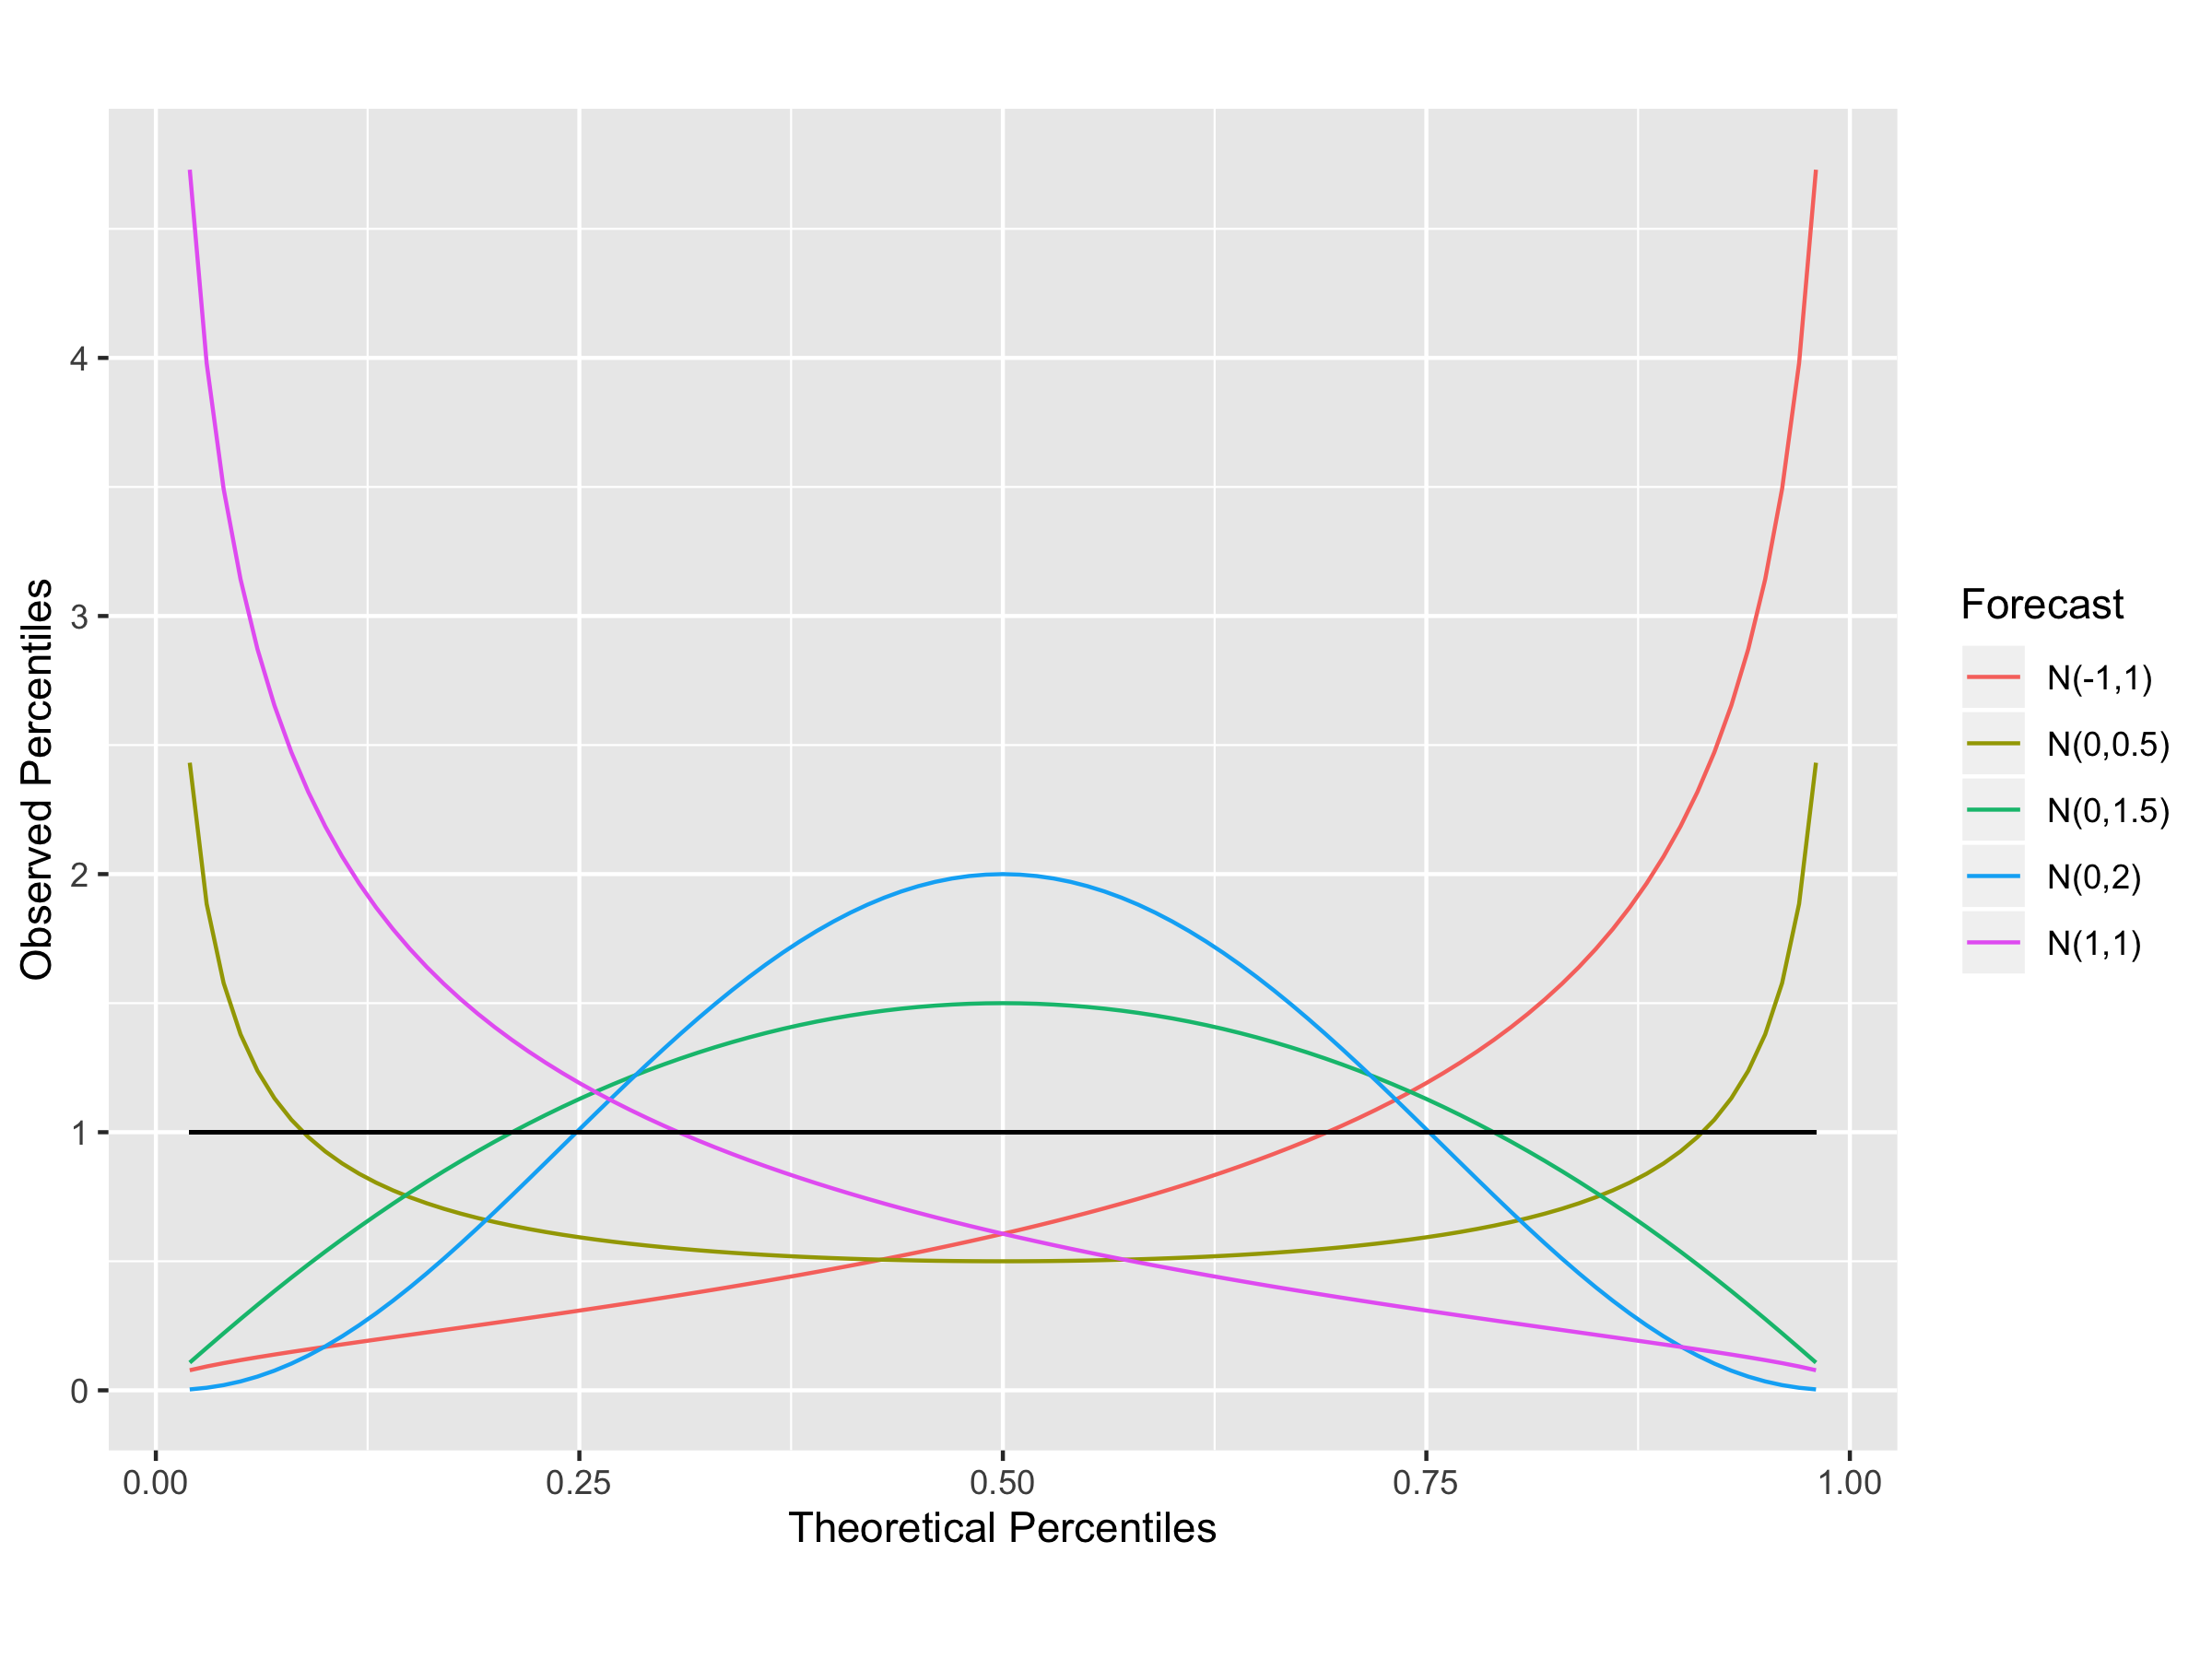
\includegraphics[width=0.7\textwidth]{rumack1.png}
\vspace{-15pt}
\caption{Densities of PIT distributions for several simple normal forecasters,
  when the true target distribution is $N(0,1)$, from
  \citet{rumack2022recalibrating}.}  
\label{fig:rumack1}   

\bigskip\medskip

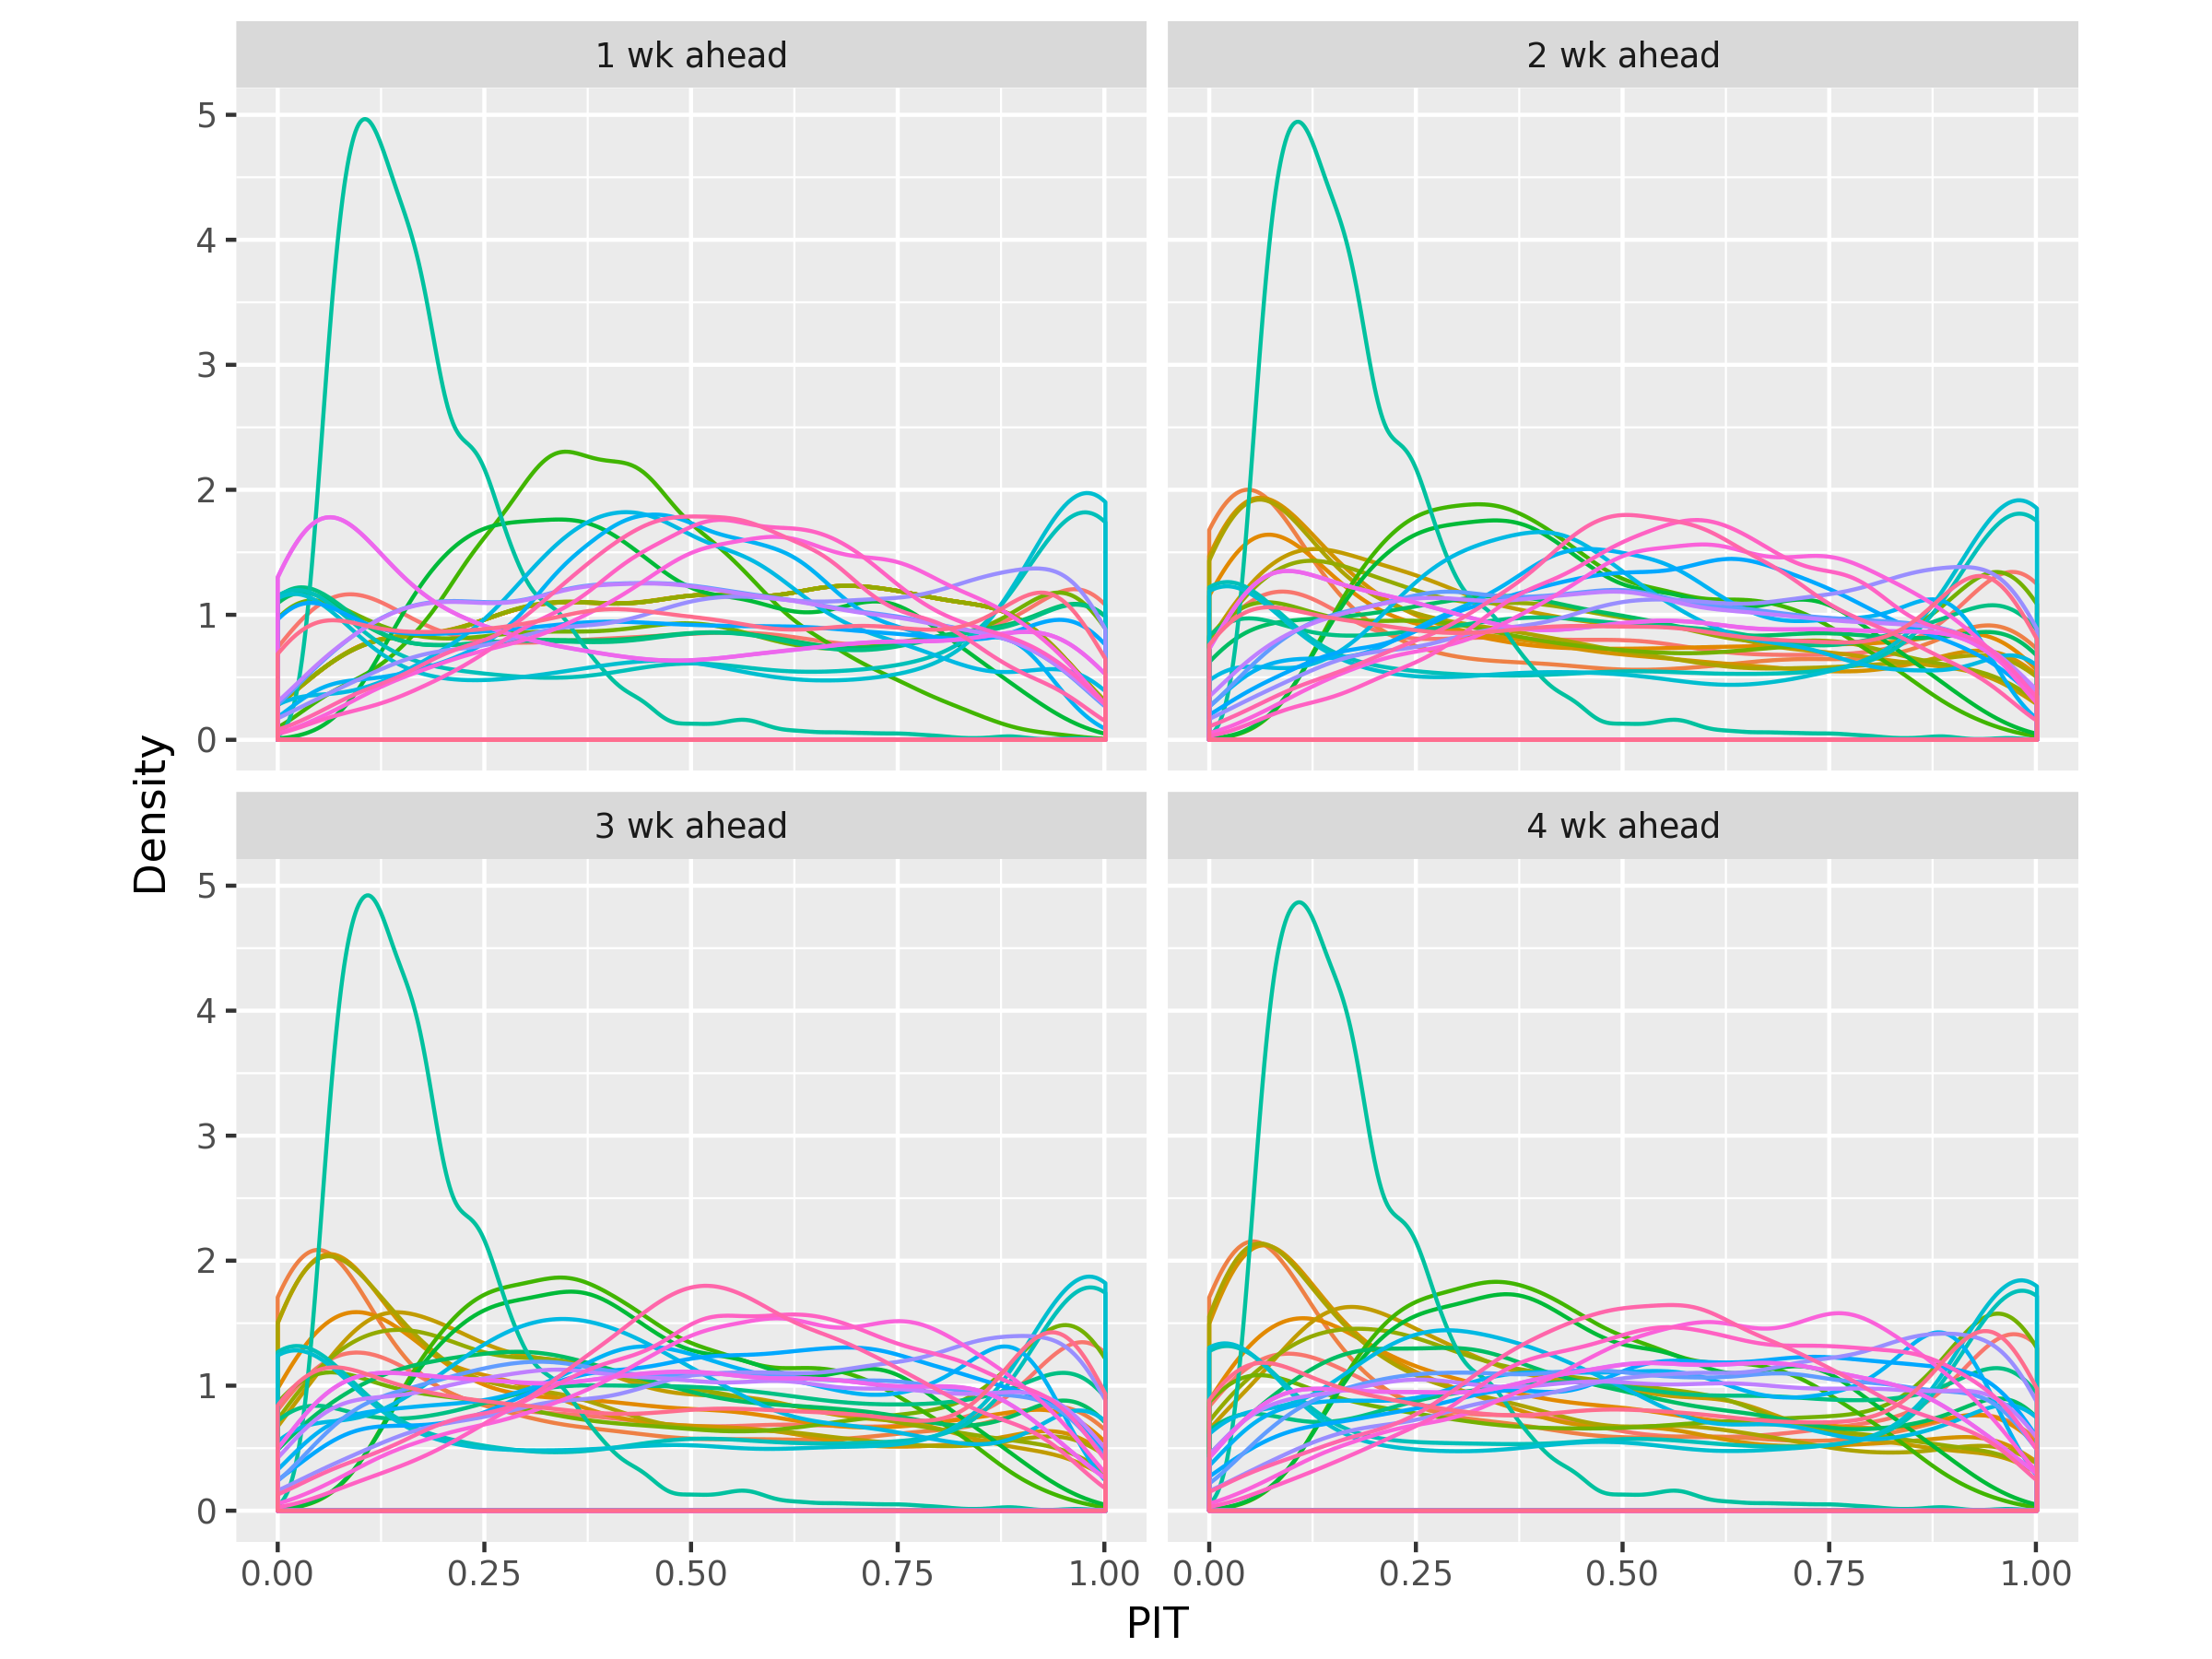
\includegraphics[width=0.85\textwidth]{rumack2.png}
\caption{Densities of PIT distributions from 27 forecasters submitted to the
  annual FluSight challenges, from \citet{rumack2022recalibrating}. These are
  seasonal influenza forecasting challenges held by CDC, spanning 9 seasons
  (2010-11 to 2018-19). The PIT densities fall mostly into one of two
  categories: overdispersed with a peak around 0.5, and underdispersed with
  peaks at around 0 and 1. (The outlier with a peak at 0.1 is the PIT density of
  a simple baseline forecaster.).}            
\label{fig:rumack2}
\end{figure}

\item Being more general than coverage, it is also harder to achieve PIT
  calibration in practice (certainly in a distribution-lean sense, without many
  assumptions). However, this is an active area of research, and we will likely
  see new advances in the next few years
\end{itemize}

\bibliographystyle{plainnat}
\bibliography{advanced}

\end{document}
